\section{Adding Functionality into \CNAME\label{sec:example}}

The following shows a sequence of figures and text of an example, where we demonstrate how to modify the code base by adding a new child process called SurvivalConstantRate. Although we will be showing adding new process functionality for a process we will explain it in a generalised way so that this can be translated into adding a new selectivity, observation, likelihood, Projection, MCMC, minimiser, time varying class etc.

To add a new process you start by going into the \path{CASAL2\CASAL2\source\processes\}. 
	
	
	\begin{figure}[!ht]
		\centering
		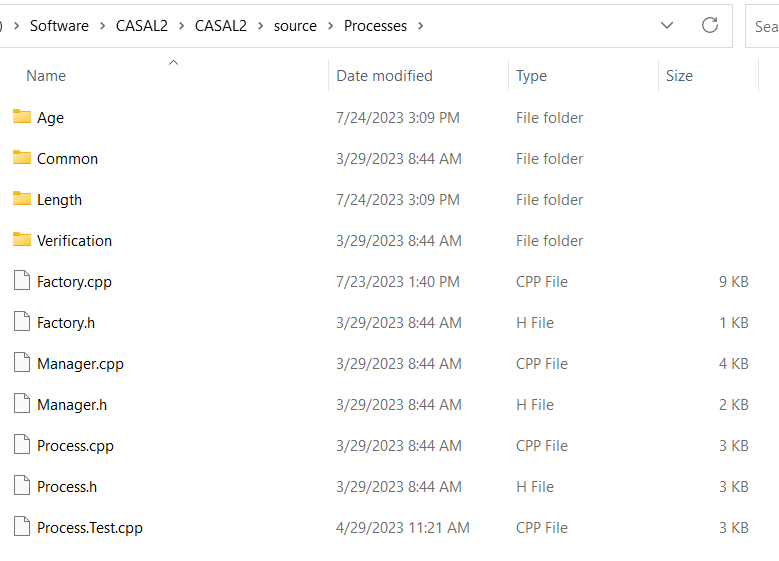
\includegraphics[scale=0.6]{Figures/adding_process1.png}
		\caption{}\label{fig:process}
	\end{figure}


This folder shown in Figure~\ref{fig:process} contains a general layout of all main classes in \CNAME. It contains a folder named \texttt{Children}, C++ source code \texttt{Factory.cpp}, \texttt{Factory.h}, \texttt{Manager.cpp}, \texttt{Manager.h}, \texttt{Process.cpp}, \texttt{Process.h}. The folder \texttt{Children} contains all the current processes implemented in \CNAME. The \texttt{Factory} source code creates all the processes during runtime. The \texttt{Manager} source code managers the class it can build pointers to specific processes to share information across classes. The \texttt{Process} source code contains base functionality that is inherited by all child classes (inheritance is a major concept in C++ and it is  advised have some knowledge of the concept). Before creating a new child look at the parent (in this example \texttt{Process.cpp}, \texttt{Process.h}), to see the functionality you don't have to add in your child because it is already done at the parent level. The following figure shows the constructor in \texttt{Process.cpp}.
\clearpage
\begin{figure}[!ht]
	\centering
	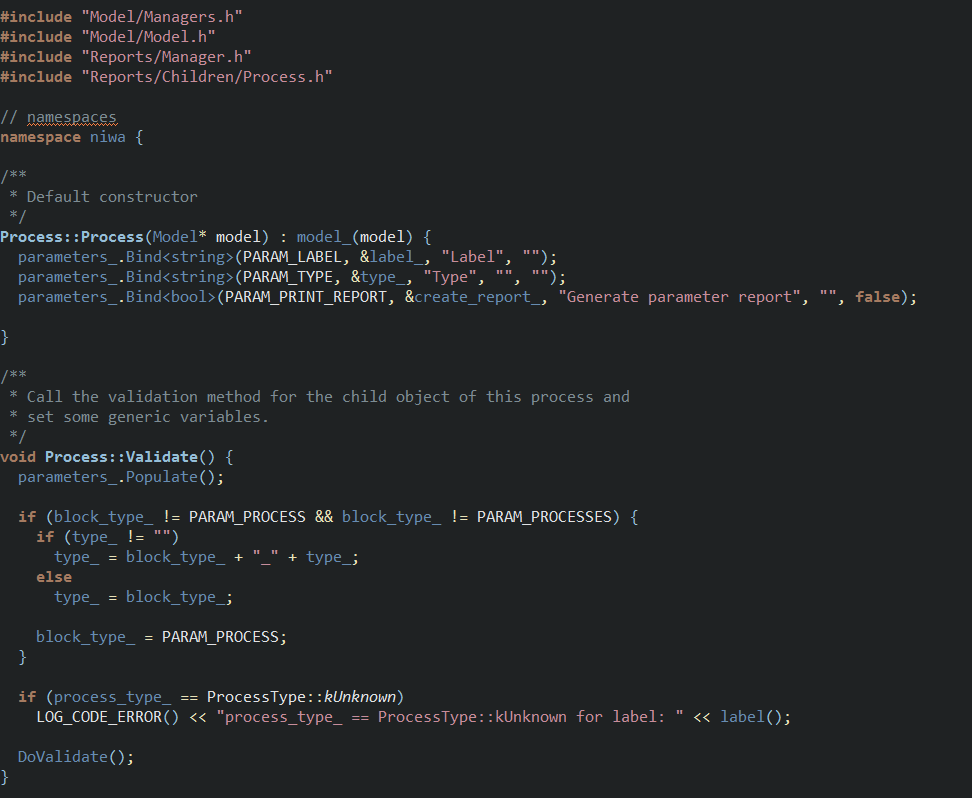
\includegraphics[scale=0.6]{Figures/add_survival1.png}
	\caption{}\label{fig:process1}
\end{figure}

From Figure~\ref{fig:process1} the process parent class does not do much it assigns a label and type for each child that will be created and a report subcommand. The point of this is to look at the parent class to reduce duplicating functionality in the child class.


We will be returning to the factory source code later but for now lets get adding a new process. Enter the \texttt{Children} folder and create C++ source code labelled \texttt{SurvivalConstantRate.cpp} and \texttt{SurvivalConstantRate.h}. I usually copy an existing process and rename it, although this is not good coding practice. It's one of those do as I say not as I do types of things.
\begin{figure}[!ht]
	\centering
	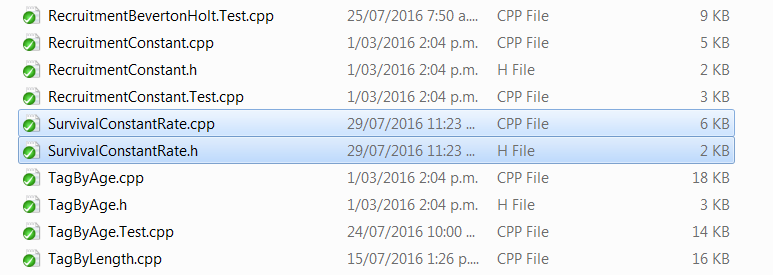
\includegraphics[scale=0.6]{Figures/add_survival.png}
	\caption{}\label{fig:process2}
\end{figure}

once you have done that for each child class you may have to write code for the following functions \texttt{DoValidate()}, \texttt{DoBuild()}, \texttt{PreExecute()}, \texttt{DoExecute()}, \texttt{PostExecute()}, \texttt{DoReset()}. To understand what these all do Figure~\ref{fig:flow} shows the state transition of \CNAME.
\raggedbottom
\begin{figure}[!ht]
	\centering
	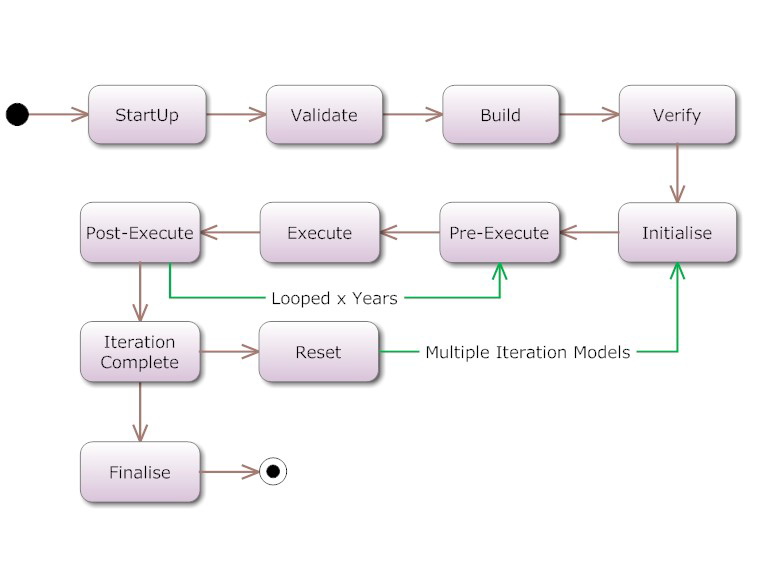
\includegraphics[scale=0.6]{Figures/State-Transition.png}
	\caption{}\label{fig:flow}
\end{figure}

Now we describe the purpose of each transition and this will give you an idea of what you should be incorporating in each function.

\paragraph*{StartUp}
The model is in the blank start and the configuration system is loading the configuration files and parsing any extra inputs.
\\
Tasks completed:
\begin{itemize}
	\item Parse command line
	\item Parse configuration file
	\item Load plugins
	\item Load estimate values from input files
\end{itemize}

\paragraph*{Validate}
All user configurations have been loaded at this point. Now the model will go through every object that has been created and check that the parameters given to them.
\\\\
This step will ensure every object in the model has sufficient parameters to be executed without causing a system fault or error in the model.
\\\\
This state will not check the values to ensure they are logical in relation to an actual model. They will only test that they exist and meet minimum requirements to execute a model.
\\\\
At the end of the validate stage each object should be internally consistent. No lookups or external references are allowed to be formed during this stage.

\paragraph*{Build}
The build phase is where the system will build relationships between objects that rely on each other. Because validation has been completed, each object in it's self-contained configuration is ok.
\\\\
This phase generally assigns values to pointers for objects so they don't need to do lookups of objects during execution phases.

\paragraph*{Verify}
At this point pre-defined configurations are checked against the model's current configuration to verify if the model makes sense logically. These are business rules being applied to the model to help ensure the output is not garbage.
\\\\
Note: This state is not executed by default and must be defined as part of the model execution.
\hl{Note: This has not been implemented.}
\paragraph*{PreExecute}
Pre-Execution happens at the beginning of a time step. This allows objects to calculate values based on the partition state before any of the other processes in the time step are executed.
\paragraph*{Execute}
This is the general work method of the model and where all of the processes will be run against the partition.
\paragraph*{PostExecute}
This is executed at the end of a time step after all of the processes and associated objects have been executed. This is typically used for things like reports and derived quantities.

\paragraph*{IterationComplete}
This is executed at the end of every model run. This is only useful when the model is in a multiple-iteration mode (e.g MCMC or Estimation). After every model iteration this state is triggered.

\paragraph*{Reset}
If the model has to run multiple iterations then the reset state is used to reset everything back in to a state where the model can be re-executed without any legacy data remaining.
\\\\
This state allows us to run multiple iterations of the model without having to re-process the configuration information or de-allocate/re-allocate large amounts of memory.


\paragraph*{Finalise}
Finalise will happen after all iterations of the model have been completed.
\pagebreak


Coming back to our example, if we look in \texttt{SurvivalConstantRate.h} we will so the following set up, as shown in Figure~\ref{fig:process_h}

\begin{figure}[!ht]
	\centering
	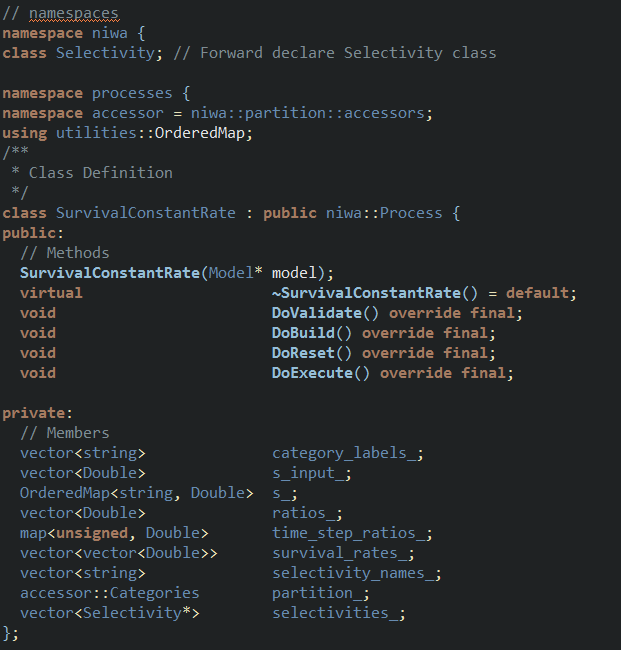
\includegraphics[scale=0.6]{Figures/process_h.png}
	\caption{}\label{fig:process_h}
\end{figure}

We can see that we are implementing \texttt{DoValidate()}, \texttt{DoBuild()}, \texttt{DoExecute()}, \texttt{DoReset()}, which are public functions and we define our variables as private. This idea of structuring classes by public, private and protected is known as encapsulation, and is another important C++ concept. Our variables will be stored in memory for the entire model run so you must make decisions on whether a variable needs to persist for the entire model run or can be temporarily created and destroyed at execution time (Note: the \_ at the end this indicates whether the variable is defined in the \texttt{.h} file or not). 
\\\\
Moving into \texttt{SurvivalConstantRate.cpp} if we look at the constructor. We can see that this describes input parameters that are supplied by the user, and which variables are estimable. This is applied by the \texttt{RegisterAsEstimable()} function.

\begin{figure}[!ht]
	\centering
	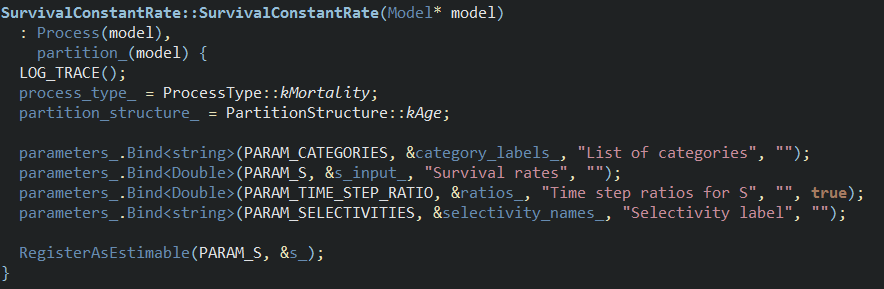
\includegraphics[scale=0.8]{Figures/constructor.png}
	\caption{}\label{fig:constructor}
\end{figure}
When you see keywords that begin with \texttt{PARAM}, for example \texttt{PARAM\_CATEGORIES}, these will be defined in \path{CASAL2\CASAL2\source\English_UK.h}

Moving on to the \texttt{DoValidate()} function in Figure~\ref{fig:validate}. The purpose of this function is to validate the users inputs and expand inputs to allow short hand syntax. You can see the annotation of what is happening in the function. This is considered one of the coding commandments \textbf{Thou shall annotate thy code}.
\begin{figure}[!ht]
	\centering
	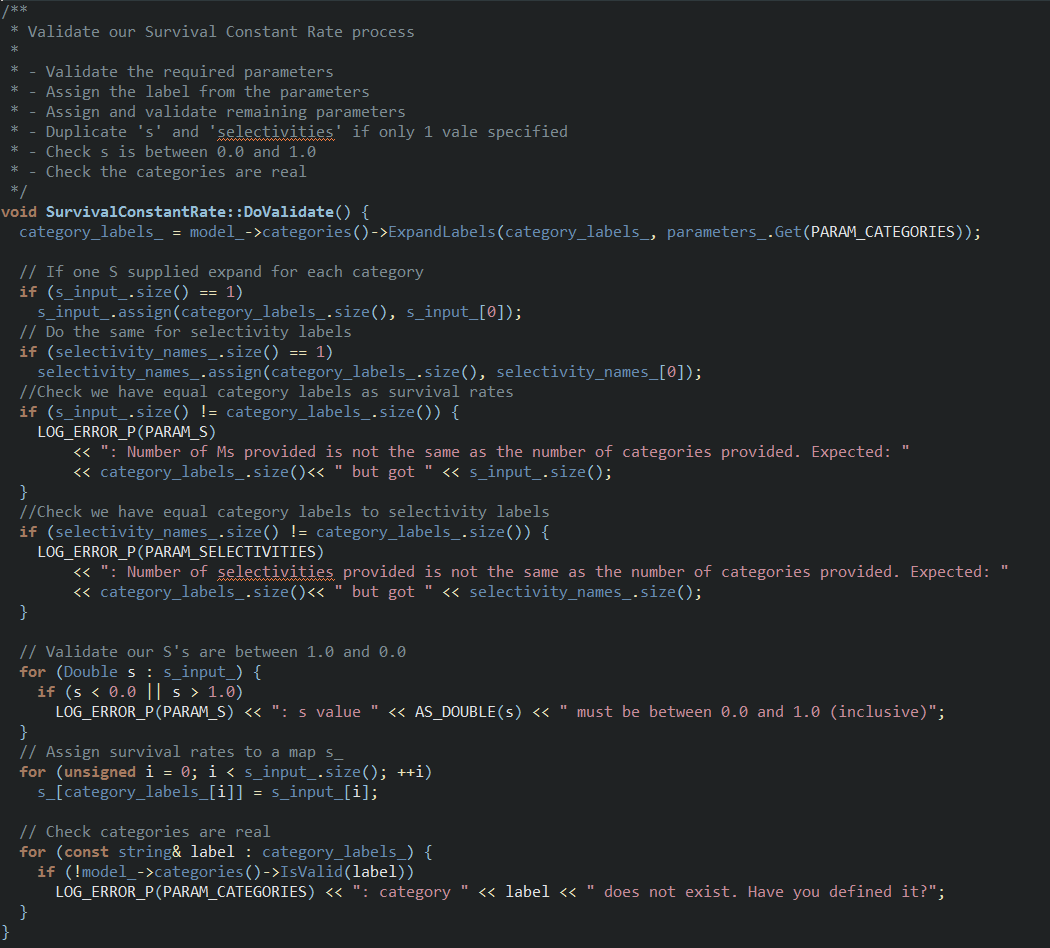
\includegraphics[scale=0.7]{Figures/validate.png}
	\caption{}\label{fig:validate}
\end{figure}

Another nice inclusion to the \CNAME\ source code is it's error checking and messages to the users. The following list is of all the allowable types of errors that \CNAME\ can perform.

\begin{itemize}
	\item \texttt{LOG\_WARNING() << "warning message";} if triggered print the warning message at the end of model run to, warn the user of a change or implication in the model.
	\item \texttt{LOG\_ERROR() << "error message";} After validate and build stop execution and print error message.
	\item \texttt{LOG\_ERROR\_P(PARAM\_KEYWORD) << "error message";} After validate and build stop execution and print error message with location of the parameter \texttt{PARAM\_KEYWORD} in the configuration files.
	\item \texttt{LOG\_FATAL()} if triggered halt execution and print error message.
	\item \texttt{LOG\_FATAL\_P(PARAM\_KEYWORD) << "error message";} If triggered stop execution and print error message with location of the \texttt{PARAM\_KEYWORD} in the configuration files.		
	\item \texttt{LOG\_CODE\_ERROR() << "error message";} if triggered quit \CNAME\ with a message like contact the development team this is a bug in the software.	
\end{itemize}

We encourage you to put these all throughout the validate and build functions to help users correctly specify models and catch silly inputs sequences.


Moving on to the \texttt{DoBuild()} function. The purpose of the build function is to create pointers and relationships with other classes that will be required during execution. For example in this process we will require access to the partition, time step and selectivity classes.

\begin{figure}[!ht]
	\centering
	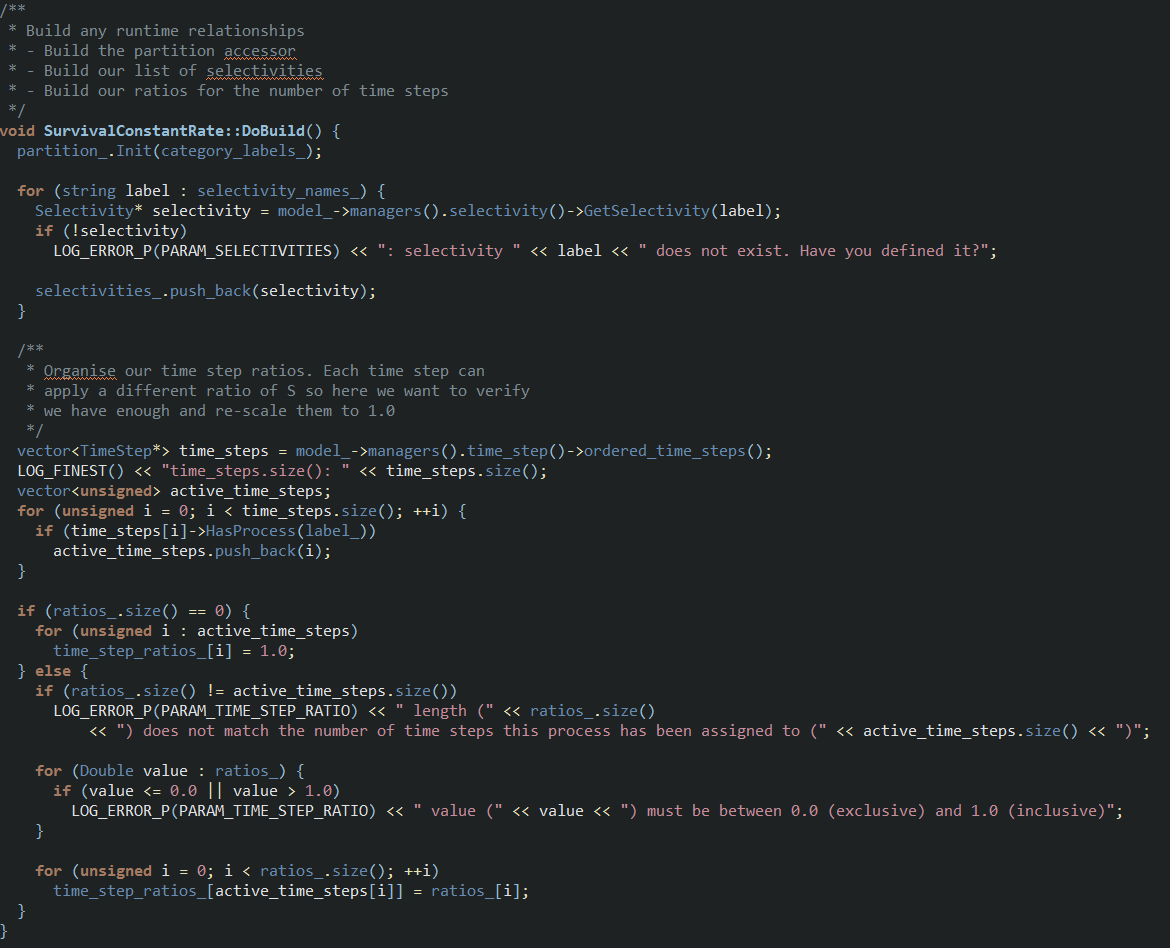
\includegraphics[scale=0.7]{Figures/Build.png}
	\caption{}\label{fig:build}
\end{figure}


Moving on to the \texttt{DoBuild()} function. This is where the action happens and we apply a survival rate to our categories.
\clearpage
\begin{figure}[!ht]
	\centering
	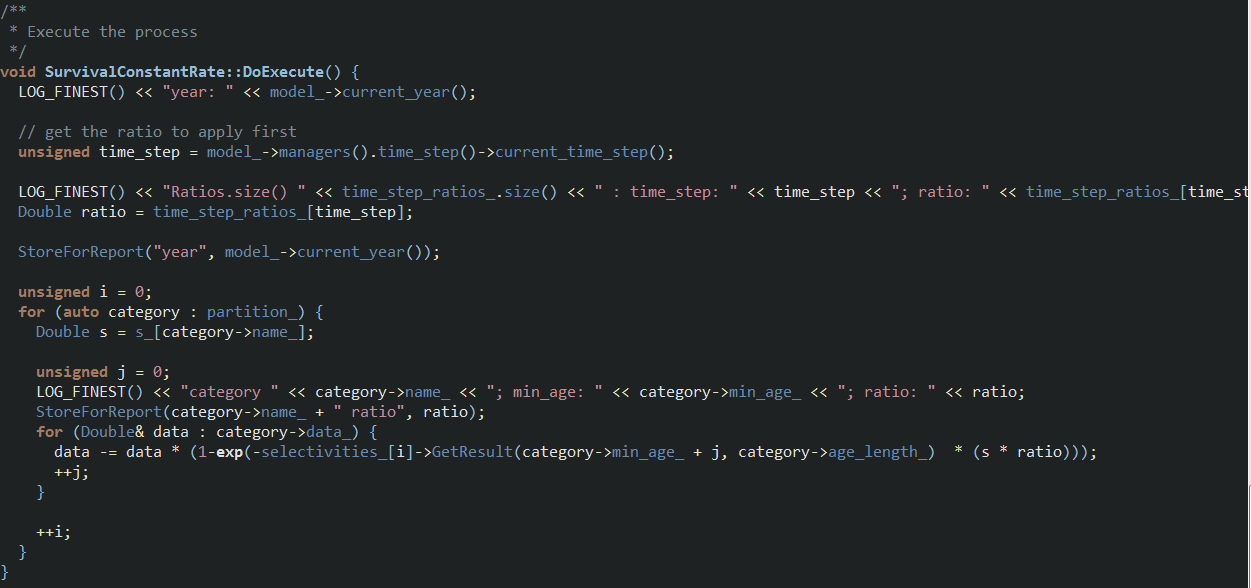
\includegraphics[scale=0.65]{Figures/execute.png}
	\caption{}\label{fig:execute}
\end{figure}

You will notice another set of logging, which is also encouraged to add all throughout the execution process. The levels of logging are described in Section~\ref{subsec:code_practive}

\paragraph*{Adding a unittest}

